\documentclass[aspectratio=169]{beamer}

\usepackage{amsmath, amssymb, amsxtra, amsthm, amsfonts}
\usetheme{moloch}
\usecolortheme{beaver}
\setbeamertemplate{footline}
{
  \leavevmode%
  \hbox{%
    \begin{beamercolorbox}[wd=.5\paperwidth,ht=2.25ex,dp=1ex,center]{author in head/foot}%
      \usebeamerfont{author in head/foot}\insertsection
    \end{beamercolorbox}%
    \begin{beamercolorbox}[wd=.5\paperwidth,ht=2.25ex,dp=1ex,right]{date in head/foot}%
      \usebeamerfont{date in head/foot}\inserttitle\hspace*{2em}
      \insertframenumber{} / \inserttotalframenumber\hspace*{2ex}
    \end{beamercolorbox}}%
  \vskip0pt%
}
\makeatother

\usepackage[english]{babel}
\usefonttheme{serif}

\usepackage{mathtools}
\usepackage{graphicx}
\usepackage{bm}
\usepackage{color}
\usepackage[dvipsnames,table]{xcolor}
\usepackage{tikz}
\usepackage{stanli}
\usepackage{verbatim}
\usepackage{tikz}
\usetikzlibrary{shapes,calc,through,3d,patterns}
\usetikzlibrary{decorations.pathreplacing}
\usetikzlibrary{arrows.meta,calc,positioning}

\usepackage{pgfplots}
\usepackage{siunitx} % For formatting numbers
\usepackage{hyperref}
\hypersetup{colorlinks=true,linkcolor=darkred}
\usepackage{multicol}
\usepackage[absolute,overlay,]{textpos}
\usepackage{pgfplots}
\pgfplotsset{width=10cm,compat=1.9}
\usepackage{subcaption}
\usepackage{multirow}
\usepackage{bbding}
\usepackage{arydshln}
\usepackage{mathtools}
\usepackage{tcolorbox}
\usepackage{animate}

\textblockorigin{80mm}{45mm}


\newtheorem{thm}{Theorem}
\newtheorem{cor}[thm]{Corollary}
\newtheorem{prop}[thm]{Proposition}
\newtheorem{lem}[thm]{Lemma}
\theoremstyle{remark}
\newtheorem*{rem}{Remark}

%Block def
\definecolor{darkred}{rgb}{0.6,0,0}
\setbeamertemplate{blocks}[rounded][shadow=false]
\setbeamercolor{block title}{bg=darkred!15,fg=black}
\setbeamercolor{block body}{bg=darkred!5,fg=black}

\setbeamercolor{itemize item}{fg=darkred}
\setbeamercolor{itemize subitem}{fg=darkred}
\setbeamercolor{itemize subsubitem}{fg=darkred}
\setbeamercolor{enumerate item}{fg=darkred}
\setbeamercolor{button}{bg=gray!30,fg=darkred}

\setbeamertemplate{itemize item}[square]
\setbeamertemplate{itemize subitem}[circle]
\setbeamertemplate{itemize subsubitem}[triangle]
\setbeamertemplate{enumerate items}[circle]
\setbeamercolor{item projected}{bg=darkred}

\newcommand{\bolddelta}{\boldsymbol\delta}
\newcommand{\boldxi}{\boldsymbol\xi}
\DeclareMathOperator*{\A}{\text{\raisebox{-0.2cm}{\Huge A}}}




\title{Eigenvalue problems of vibrations and stability}
\subtitle{Analysis of free and forced vibrations}
\author{ME473 Dynamic finite element analysis of structures}
\institute{Stefano Burzio}
\date{2025}

\begin{document}
\usenavigationsymbolstemplate{}
{\setbeamertemplate{footline}{}

  \frame{\titlepage
    \begin{tikzpicture}[overlay, remember picture]
      \node[anchor=north east, xshift=-.9cm] at (current page.north east) {
\includegraphics[width=2cm]{../images/epfl_logo.png}};
      \node[anchor=south east, xshift=-.87cm, yshift=.05cm] at (current page.south east)  {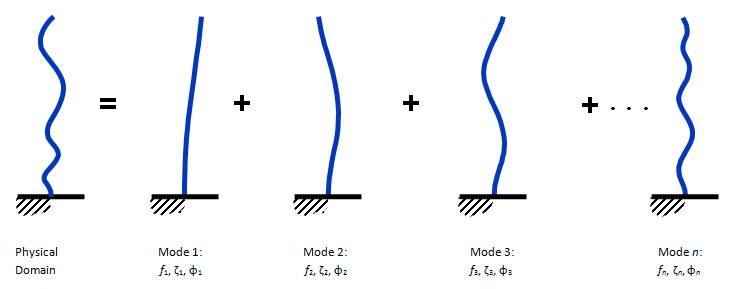
\includegraphics[height=3cm]{../images/ModalDecomposition.png}};
    \end{tikzpicture}
  }

  \begin{frame}{Where do we stand?}
    \begin{center}
      \begin{tabular}{|c|l|l|l|}
        \hline
        \rowcolor{darkred!20}\textbf{Week} & \textbf{Module}                                & \textbf{Lecture topic}             & \textbf{Mini-projects} \\
        \hline

        1                                  & \multirow{6}{7em}{Linear elastodynamics}       & Strong and weak forms              &                        \\ \cline{1-1} \cline{3-4}
        2                                  &                                                & Galerkin method                    &                        \\ \cline{1-1} \cline{3-4}
        3                                  &                                                & Finite element method              & Groups formation       \\ \cline{1-1} \cline{3-4}
        4                                  &                                                & Systematization of the procedure   & Project 1 statement    \\
        \cline{1-1} \cline{3-4}
        5                                  &                                                & 3d elements, numerical integration &                        \\
        \hline
        6                                  & \multirow{5}{7em}{Special structural elements} & Bars and trusses                   &                        \\
        \cline{1-1} \cline{3-4} 7          &                                                & Planar beams                       & Project 1 submission   \\
        \cline{1-1} \cline{3-4} 8          &                                                & Frames and grids                   & Project 2 statement    \\

        \cline{1-1} \cline{3-4} 9          &                                                & Kirchhoff-Love plates              &                        \\
        \cline{1-1} \cline{3-4}
        10                                 &                                                & Reissner-Mindlin plates            &                        \\
        \cline{1-1} \cline{3-4}
        11                                 &                                                & Shells                             & Project 2 submission   \\
        \hline
        12                                 & \multirow{1}{7em}{Free and forced vibrations}  & Analysis of free vibrations        & Project 3 statement    \\
                                           &                                                &                                    &                        \\
        \hline
      \end{tabular}
    \end{center}
    \vspace{1cm}
  \end{frame}

  \begin{frame}
    \textbf{\large Summary}
    \begin{itemize}
      \item Recap week 11
      \item Modal properties of conservative systems
      \item Example: Rayleigh's quotient for axial vibrations of a free-free bar
      \item Numerical modal extraction algorithms for conservative systems
    \end{itemize}
    \vspace{.5cm}

    \textbf{\large Recommended readings}
    \begin{itemize}
      \item[(N)] Neto et al., Engineering Computation of Structures (chap. 2.5)
      \item[(P)] Petyt, Introduction to finite element vibration analysis (chap. 11)
      \item[(G)] Gmür, Dynamique des structures (§4.1 and §4.2)
    \end{itemize}
  \end{frame}
}

\section{Recap week 11 \\ Vibrations of shells}
 {\setbeamercolor{background canvas}{bg=darkred!5}
  \setbeamercolor{block body}{bg=darkred!5,fg=black}
  \begin{frame}{Shell element}
    \begin{center}
      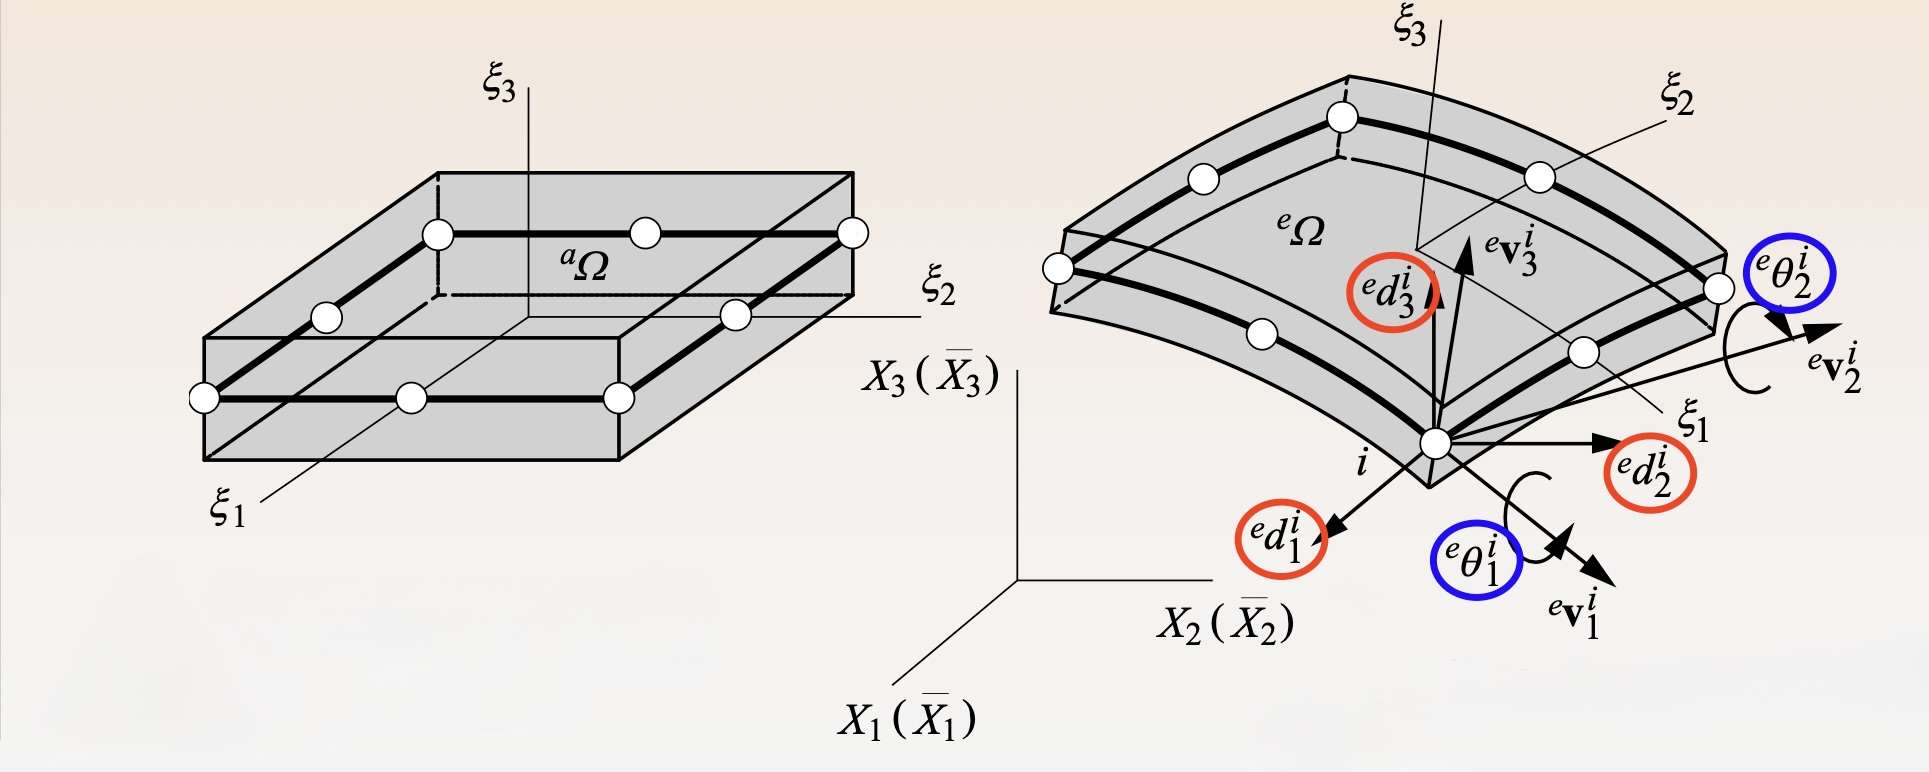
\includegraphics[height=4cm]{../images/shell6.jpeg}
    \end{center}
    \begin{itemize}
      \item have 5 DOFs per node, no rotation ${}^e\theta_3^i$.
      \item lead to huge computational time savings since allow modeling with fewer mesh elements.
      \item less prone to negative Jacobian errors which might occur when using extremely thin 3d solid elements.
    \end{itemize}
  \end{frame}

  \begin{frame}{Shape functions matrix}
    \begin{block}{}\vspace{-0.5cm}
      \begin{align*}
        \mathbf u^h(\boldxi) & =\sum_{i=1}^{{}^ep}{}^ah_i(\xi_1,\xi_2)\left[{}^e{\mathbf d}^i+\frac{1}{2}\xi_3{}^e t_3^i\left(-{}^e\theta_1^i{}^e\mathbf v_2^i+{}^e\theta_2^i{}^e\mathbf v_1^i\right)\right] \\[10pt]
                             & =\sum_{i=1}^{{}^ep}{}^a\mathbf H_i(\boldxi){}^e\mathbf q^i(t)                                                                                                                 \\[10pt]
                             & =\sum_{i=1}^{{}^ep}\underbrace{\left[
            \begin{array}{ccc|cc}
              {}^a h_i                                                 & 0                                                       & 0        &
              -\dfrac{1}{2}\xi_3{}^e t_3^i \, {}^a h_i \, {}^ev_{21}^i & \dfrac{1}{2}\xi_3{}^e t_3^i \, {}^a h_i \, {}^ev_{11}^i                                                                                                                             \\[7pt]
              0                                                        & {}^a h_i                                                & 0        & -\dfrac{1}{2}\xi_3{}^e t_3^i \, {}^a h_i \, v_{22}^i & \dfrac{1}{2}\xi_3{}^e t_3^i \, {}^a h_i \, {}^ev_{12}^i \\[7pt]
              0                                                        & 0                                                       & {}^a h_i &
              -\dfrac{1}{2}\xi_3{}^e t_3^i \, {}^a h_i \, {}^ev_{23}^i & \dfrac{1}{2}\xi_3{}^e t_3^i \, {}^a h_i  \,{}^ev_{13}^i
            \end{array}
            \right]}_\text{${}^a\mathbf H_i$}
        \underbrace{\begin{bmatrix}
                        {}^e{d}^i_1 \\[2pt] {}^e{d}^i_2 \\[2pt] {}^e{d}^i_3 \\[2pt] {}^e{\theta}^i_1 \\[2pt] {}^e{\theta}^i_2
                      \end{bmatrix}}_\text{${}^e\mathbf q^i$}
      \end{align*}
    \end{block}
  \end{frame}

  \begin{frame}{Example: 8 nodes quadrangular shell element}
    \begin{center}
      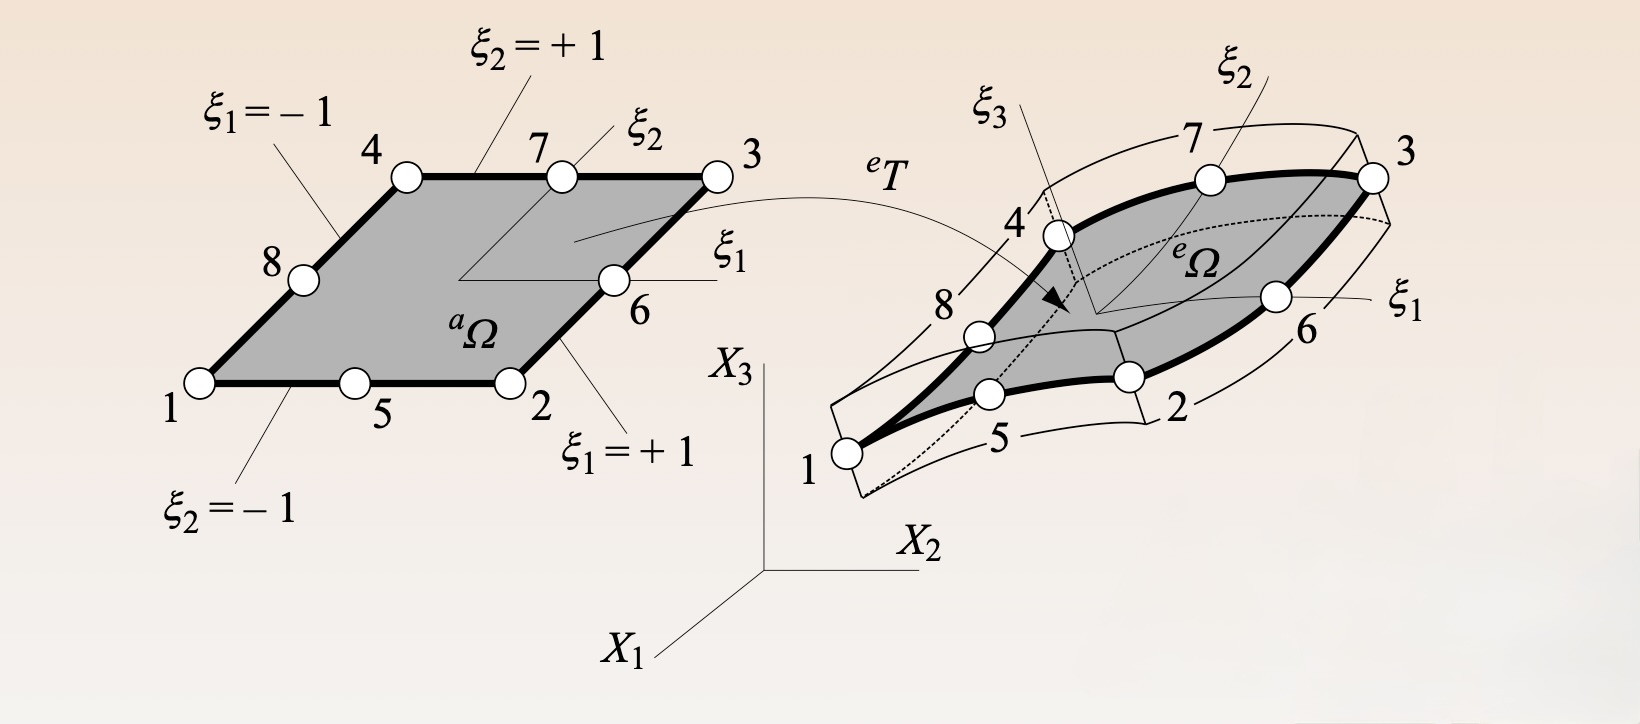
\includegraphics[height=5.5cm]{../images/shellQuad8.jpeg}
    \end{center}
  \end{frame}
 }

\section{Analysis of free vibrations}

\begin{frame}{Free vibrations of non-rotating conservative systems}
  The discretization of linear three-dimensional elastodynamics, as well as the analysis of vibrations in beams, plates and shells, all lead to a system of ODE:
  \[
    \mathbf{M} \ddot{\mathbf{q}}(t) + \mathbf{K} \mathbf{q}(t) = \mathbf{r}(t),
  \]
  \begin{columns}[T]
    \begin{column}{.4\textwidth}
      \vspace{-1cm}
      \begin{center}
        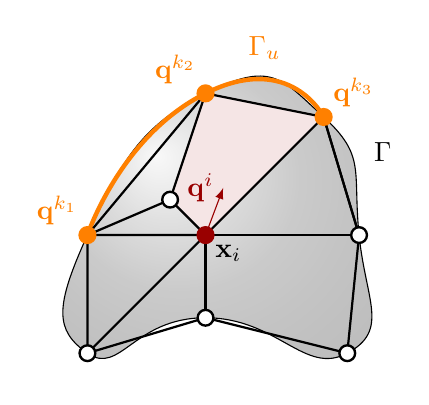
\begin{tikzpicture}[scale=1.5]
          %\draw[step=1.0,black,thin] (0,0) grid (4,4);
          % Draw the potato-like shape
          \shade [ball color= gray!90!black, opacity=.3] plot [thick,smooth cycle, tension=1] coordinates  {(1,2) (2,3.2) (3,3) (3.3,2) (3.2,1) (2,1.3) (1,1)};
          \draw[thin] plot [smooth cycle, tension=1] coordinates {(1,2) (2,3.2) (3,3) (3.3,2) (3.2,1) (2,1.3) (1,1)};
          \draw[ultra thick, orange] plot [smooth, tension=1.3] coordinates {(1,2) (2,3.2) (3,3)};
          \draw[fill=darkred!30,thick,darkred!10] (2,2) -- (3,3) -- (2,3.2) -- (1.7,2.3) -- cycle;
          \node[below right] at (2,2) {$\mathbf x_i$};
          \draw[-latex,darkred] (2,2) -- (2.15,2.4) node[darkred, left]{$\mathbf q^i$};
          % Label the boundary Gamma
          \node at (3.5,2.7) {$\Gamma$};
          \node[orange, above] at (2.5,3.4) {$\Gamma_u$};
          \draw[thick] (1,2) -- (2,3.2) -- (3,3) -- (3.3,2) -- (3.2,1) -- (2,1.3) -- (1,1) -- cycle;
          \draw[thick] (1,2) -- (2,2) -- (3,3) -- (3.3,2);
          \draw[thick] (2,1.3) -- (2,2) -- (3.3,2);
          \draw[thick] (1,1) -- (2,2) -- (1.7,2.3) -- (2,3.2);
          \draw[thick] (1.7,2.3) -- (1,2);
          \node[darkred,draw,shape=circle,fill=darkred,minimum size=2mm,line width=0.3mm,inner sep=0] at (2,2) {};
          \node[draw,shape=circle,fill=white,minimum size=2mm,line width=0.3mm,inner sep=0] at (1,1) {};
          \node[orange,draw,shape=circle,fill=orange,minimum size=2mm,line width=0.3mm,inner sep=0] at (1,2) {};
          \node[draw,shape=circle,fill=white,minimum size=2mm,line width=0.3mm,inner sep=0] at (2,1.3) {};
          \node[orange,draw,shape=circle,fill=orange,minimum size=2mm,line width=0.3mm,inner sep=0] at (2,3.2) {};
          \node[draw,shape=circle,fill=white,minimum size=2mm,line width=0.3mm,inner sep=0] at (1.7,2.3) {};
          \node[orange,draw,shape=circle,fill=orange,minimum size=2mm,line width=0.3mm,inner sep=0] at (3,3) {};
          \node[draw,shape=circle,fill=white,minimum size=2mm,line width=0.3mm,inner sep=0] at (3.2,1) {};
          \node[draw,shape=circle,fill=white,minimum size=2mm,line width=0.3mm,inner sep=0] at (3.3,2) {};
          \node[orange,above left] at (1,2) {$\mathbf q^{k_1}$};
          \node[orange,above left] at (2,3.2) {$\mathbf q^{k_2}$};
          \node[orange,above right] at (3,3) {$\mathbf q^{k_3}$};
        \end{tikzpicture}
      \end{center}
    \end{column}
    \begin{column}{.65\textwidth}
      \vspace{-0.9cm}
      \begin{block}{}
        \textbf{Free vibration:} no external forcing is applied, i.e.   $\mathbf{r}(t) = \mathbf{0}.$
      \end{block}
      \begin{itemize}
        \item Generalized nodal displacements: $$\mathbf q(t)=[\mathbf q^1(t),\dots, \mathbf q^n(t)]^T.$$
        \item \textbf{Boundary conditions:} $\mathbf q^k=\hat{\mathbf q}^k$ for all $k$ such that $\mathbf x_k\in\Gamma_u$.
        \item  \textbf{Initial conditions:} $\mathbf q(0)=\mathbf u_0$ and $\dot{\mathbf q}(0)=\mathbf v_0$
      \end{itemize}
    \end{column}
  \end{columns}
\end{frame}

\begin{frame}{Harmonic response}
  \begin{block}{}
    The solution for a free and undamped discrete vibration problem
    $$\mathbf{M} \ddot{\mathbf{q}}(t) + \mathbf{K} \mathbf{q}(t) = \mathbf{0}$$
    is sinusoidal, described via an harmonic function:
    $$\mathbf q(t)=\alpha \mathbf p \cos(\omega t+\varphi)$$
    \begin{multicols}{2}
      \begin{itemize}
        \item \(\mathbf{p}\): mode shape (modal vector)
        \item \(\omega\): natural frequency
        \item \(\varphi\): phase
        \item \(\alpha\): scaling factor
      \end{itemize}
    \end{multicols}
  \end{block}
  \begin{itemize}
    \item  \textcolor{darkred}{\textbf{Solutions are defined up to a scalar factor: $\alpha$.}}
    \item Three scalars unknowns $\alpha$, $\omega$, $\varphi$  and one unknown vector $\mathbf{p}$.
  \end{itemize}
\end{frame}

\begin{frame}{Generalized eigenvalue problem}
  Substituting the proposed ansatz into the equation of motion yields a generalized eigenvalue problem:
  \vspace{-0.2cm}
  \begin{align*}
    \alpha & (\mathbf{K} - \omega^2 \mathbf{M}) \mathbf{p} \cos(\omega t - \varphi)  = 0        \\
           & (\mathbf{K} - \omega^2 \mathbf{M}) \mathbf{p}                                  = 0
  \end{align*}
  \vspace{-0.8cm}
  \begin{block}{}
    \textbf{Solving the eigenvalue problem:}
    \begin{itemize}
      \item \emph{Eigenvalue}: $\lambda_j=\omega_j^2$ are the roots of the characteristic polynomial:
            $$\text{det}(\mathbf K-\omega^2\mathbf M)=0.$$
      \item \emph{Eigenvector}: $\mathbf p_j$ are the solution of the equation
            $$(\mathbf{K} - \lambda_j \mathbf{M})\mathbf p_j=\mathbf 0.$$
    \end{itemize}
  \end{block}
\end{frame}


\begin{frame}{General solution via modal superposition}
  \begin{itemize}
    \item Once the set of eigenvalue-eigenvector pairs \((\omega_j^2, \mathbf{p}_j)\) have been determined, the linearity of the system allows the general solution to be expressed as a superposition of modal contributions:
          \[
            \mathbf{q}(t) = \sum_{j=1}^n \alpha_j \, \mathbf{p}_j \cos(\omega_j t + \varphi_j)
          \]
    \item The constants \(\alpha_j\) and \(\varphi_j\) are determined from the initial conditions: $\mathbf{q}(0) = \mathbf{u}_0$ and $\dot{\mathbf{q}}(0) = \mathbf{v}_0$ leading to the system:
          \begin{align*}
            \sum_{j=1}^n \alpha_j \mathbf{p}_j \cos(\varphi_j)          & = \mathbf{u}_0  \\
            \sum_{j=1}^n \alpha_j \omega_j \mathbf{p}_j \sin(\varphi_j) & = -\mathbf{v}_0
          \end{align*}
  \end{itemize}
\end{frame}

\section{Fundamental properties of generalized eigenvalue problem}

\begin{frame}{Spectral property}
  \begin{block}{}
    \begin{itemize}
      \item If both $\mathbf{K}$ and $\mathbf{M}$ are symmetric and strictly positive definite, then all eigenvalues $\lambda_j$ of the generalized eigenvalue problem
            $$\mathbf{K} \mathbf{p}_j = \lambda_j \mathbf{M} \mathbf{p}_j$$
            are real and positive.
      \item Thus we can define the angular frequencies
            $$\omega_j=\sqrt{\lambda_j}$$
            and
            $$0<\omega_1\leq \omega_2\leq\omega_3\leq\dots\leq\omega_n.$$
    \end{itemize}
  \end{block}
\end{frame}

{\setbeamercolor{background canvas}{bg=darkred}
\setbeamercolor{block body}{bg=darkred,fg=white}
\setbeamercolor{itemize item}{fg=white}
\setbeamercolor{itemize/enumerate body}{fg=white}
\color{white}
\begin{frame}{Rigid body modes}
  In the semi-discrete weak form obtained via finite element discretization:
  \begin{itemize}
    \item The \textbf{mass matrix} \( \mathbf{M} \) is symmetric and strictly positive definite.
    \item The \textbf{stiffness matrix} \( \mathbf{K} \) is symmetric and positive semi-definite:
          \[
            \mathbf{K} \mathbf{p} = \mathbf{0} \quad \text{for certain nonzero vectors } \mathbf{p}.
          \]
  \end{itemize}
  Consequently, the eigenvalues \( \omega_j^2 \) of the generalized eigenvalue problem are all real and non-negative:
  \[
    0 \,\leq\, \omega_1 \leq \omega_2 \leq \dots \leq \omega_n.
  \]

  \begin{tcolorbox}[colback=darkred!10,colframe=darkred!40!black]
    \textbf{Rigid body modes:} zero eigenvalues (i.e., \( \omega_j = 0 \)) correspond to \emph{rigid body motions}, where the system undergoes displacement without internal deformation.
  \end{tcolorbox}
\end{frame}
}

\begin{frame}{Spectral offset technique}
  \begin{block}{}
    To ensure that the stiffness matrix is \emph{strictly} positive definite, a \textbf{spectral shift} strategy is employed. Given \( \sigma > 0 \), define the modified stiffness matrix as:
    \[
      \mathbf{K}_\sigma = \mathbf{K} + \sigma \mathbf{M}
    \]
  \end{block}
  \begin{itemize}
    \item Consider the offset eigenvalue problem:
          $            (\mathbf{K}_\sigma - \lambda_\sigma \mathbf{M}) \mathbf{p} = \mathbf{0}
          $
    \item Substituting the definition of \( \mathbf{K}_\sigma \):
          \[
            (\mathbf{K} + \sigma \mathbf{M} - \lambda_\sigma \mathbf{M}) \mathbf{p}
            = (\mathbf{K} + (\sigma - \lambda_\sigma)\mathbf{M}) \mathbf{p} = \mathbf{0}
          \]
    \item Comparing with \( (\mathbf{K} -\lambda \mathbf{M}) \mathbf{p}=\mathbf 0 \), we identify: $\lambda_\sigma = \lambda+\sigma > 0$.
  \end{itemize}
  \begin{tcolorbox}[colback=darkred!10,colframe=darkred!40!black]
    \textbf{Eigenvalues are shifted by \( \sigma \), but the eigenvectors remain the same.}
    $$\textbf{\textit{Empirical rule:}} \qquad \sigma\approx \frac{1}{100}\frac{\text{tr}(\mathbf K)}{\text{tr}(\mathbf M)}$$
  \end{tcolorbox}
\end{frame}

\begin{frame}{Orthogonality of mode shapes}
  \begin{block}{}
    Let $\mathbf p_i$ and $\mathbf p_j$ two eigenvectors corresponding to two \emph{distinct} eigenvalues $\lambda_i$ and $\lambda_j$, then
    $$
      \mathbf p_i^T\mathbf M\mathbf p_j  =0
      \qquad\text{and}\qquad
      \mathbf p_i^T\mathbf K\mathbf p_j  =0\qquad\ (i\neq j).
    $$
  \end{block}
  \emph{Consequence:} two different harmonic responses:
  $$\mathbf q_i(t)=\alpha_i \mathbf p_i \cos(\omega_i t+\varphi_i)\qquad \text{and}\qquad \mathbf q_j(t)=\alpha_j \mathbf p_j \cos(\omega_j t+\varphi_j)$$
  are $\mathbf M$- and $\mathbf K$-orthogonal:
  $$\mathbf q_i^T\mathbf M\mathbf q_j=0\qquad\text{and}\qquad \mathbf q_i^T\mathbf K\mathbf q_j=0.$$
  \vspace{-0.5cm}
  \begin{block}{}
    The virtual work of inertial and elastic forces of a given mode, along the displacement given by a different mode, is zero.
  \end{block}
\end{frame}

\begin{frame}{Normalization of mode shapes}
  \begin{block}{}
    Let $\mathbf p_i$ and $\mathbf p_j$ two eigenvectors corresponding to the eigenvalues $\lambda_i$ and $\lambda_j$, then
    $$
      \mathbf p_i^T\mathbf M\mathbf p_j  =\mu_i \delta_{ij}
      \qquad\text{and}\qquad
      \mathbf p_i^T\mathbf K\mathbf p_j  =\kappa_i\delta_{ij}
    $$
    where
    \begin{itemize}
      \item $\mu_i=$ modal mass of mode $i$,
      \item $\kappa_i=$ modal stiffness of mode $i$,
      \item $\delta_{ij}=$ Kronecker delta.
    \end{itemize}
    \textbf{Usual normalization choice: orthonormalization}
    \[
      \mu_i = 1 \qquad  \Rightarrow \qquad \lambda_i = \frac{\kappa_i}{\mu_i} = \omega_i^2.
    \]
  \end{block}
\end{frame}

{\setbeamercolor{background canvas}{bg=darkred}
\setbeamercolor{block body}{bg=darkred,fg=white}
\setbeamercolor{itemize item}{fg=white}
\setbeamercolor{itemize/enumerate body}{fg=white}
\color{white}
\begin{frame}{Orthonormalization of mode shapes}
  \vspace{-0.2cm}
  \begin{block}{}
    Let $\mathbf p_i$ and $\mathbf p_j$ two eigenvectors corresponding to the  eigenvalues $\lambda_i$ and $\lambda_j$, then
    $$
      \mathbf p_i^T\mathbf M\mathbf p_j  =\delta_{ij}
      \qquad\text{and}\qquad
      \mathbf p_i^T\mathbf K\mathbf p_j  =\omega_i^2\delta_{ij}
    $$
    where $\delta_{ij}$ represent Kronecker symbol.
  \end{block}
  \vspace{-0.3cm}
  \begin{tcolorbox}[colback=darkred!10,colframe=darkred!40!black]
    We store the modal vectors $\mathbf p_i$ in a so-called \emph{modal matrix} $\mathbf P$:
    $$\mathbf P=\left[ \begin{array}{c;{2pt/2pt}c;{2pt/2pt}c;{2pt/2pt}c}
          \mathbf p_{1} & \mathbf p_{2} & \dots & \mathbf p_{n} \\
        \end{array}\right]$$
    then
    $$  \mathbf P^T\mathbf M\mathbf P  =\mathbf I       \qquad\text{and}\qquad
      \mathbf P^T\mathbf K\mathbf P  =\mathbf\Lambda$$
    where $\mathbf I$ is the identity matrix of order $n$ and $\mathbf\Lambda$ the spectral matrix:
    $$\mathbf\Lambda=\text{diag}(\lambda_1,\dots,\lambda_n)=\text{diag}(\omega_1^2,\dots,\omega_n^2).$$
  \end{tcolorbox}
\end{frame}
}

\section{Example: longitudinal vibrations of free-free bar}

\begin{frame}{Longitudinal vibrations of free-free bar}
  Consider a free-free bar discretized by one bilinear element.
  \begin{columns}
    \column{0.65\textwidth}
    \begin{center}
      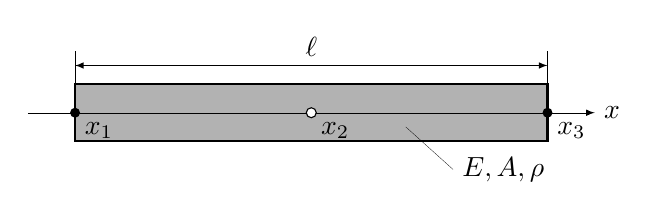
\begin{tikzpicture}[scale=0.6]
        % Draw the rectangle
        \filldraw[fill=gray!60, draw=black,thick] (0,-0.6) rectangle (10,0.6);
        %axis
        \draw[-latex, ultra thin] (-1,0) -- (11,0) node[right]{$x$};
        % length
        \draw[ultra thin] (10,0) -- (10, 1.3) ;
        \draw[ultra thin] (0,0) -- (0,1.3);
        \draw[latex-latex, ultra thin]  (0,1)  to node[sloped,midway,above] {$\ell$}(10,1) ;
        \draw[ultra thin]  (7,-0.3) -- (8,-1.2) node[right]{$E,A,\rho$};

        \fill (0,0) circle (3pt) node[below right] {$x_1$};
        \fill (10,0) circle (3pt) node[below right] {$x_3$};
        \draw[fill=white, draw=black] (5,0) circle (3pt) node[below right] {$x_2$};
      \end{tikzpicture}
    \end{center}
    \column{0.5\textwidth}
    {\small \begin{itemize}
        \item $\ell$ length
        \item $A$ cross-sectional area
        \item $E$ Young's modulus
        \item $\rho$ material density
      \end{itemize}}
  \end{columns}
  \begin{block}{}
    \textbf{Objectives}:
    \begin{enumerate}
      \item compute the approximated natural frequencies and corresponding mode shapes,
      \item verify the presence of a rigid body mode,
      \item check the orthonormality of the mode shapes.
    \end{enumerate}
  \end{block}
\end{frame}

\begin{frame}{MATLAB example - longitudinal vibrations of free-free bar}
  \begin{center}
    \href{https://drive.mathworks.com/sharing/6a9792ef-d0a7-4aca-a1d0-8b1862b0ac3b}{\beamergotobutton{Go to Matlab Drive}}
  \end{center}
\end{frame}

\section{Eigenproblem solution methods}

\begin{frame}{Transformation to standard form by inversion}
  \vspace{-0.5cm}
  \begin{center}
    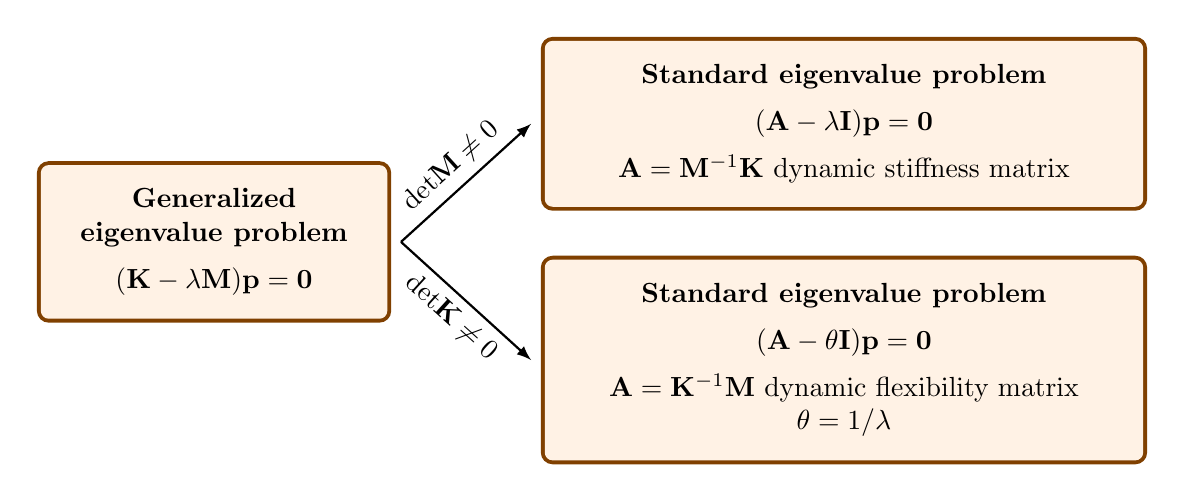
\begin{tikzpicture}
      \node (gev) at (-4,0) {
        \begin{tcolorbox}[colframe=orange!50!black, colback=orange!10, coltitle=black, rounded corners,width=4.5cm]
          \centering \textbf{Generalized eigenvalue problem} \\[5pt] $(\mathbf{K} - \lambda \mathbf{M})\mathbf p=\mathbf 0$
        \end{tcolorbox}
      };

      \node (sev1) at (4,1.5) {
        \begin{tcolorbox}[colframe=orange!50!black, colback=orange!10, coltitle=black, rounded corners,width=7.7cm]
          \centering \textbf{Standard eigenvalue problem} \\[5pt]  $(\mathbf A - \lambda \mathbf{I})\mathbf p=\mathbf 0$ \\[5pt]
          $\mathbf{A}=\mathbf{M}^{-1}\mathbf{K}$ dynamic stiffness matrix
        \end{tcolorbox}
      };

      \node (sev2) at (4,-1.5) {
        \begin{tcolorbox}[colframe=orange!50!black, colback=orange!10, coltitle=black, rounded corners,width=7.7cm]
          \centering \textbf{Standard eigenvalue problem} \\[5pt]  $(\mathbf A - \theta \mathbf{I})\mathbf p=\mathbf 0$ \\[5pt]
          $\mathbf{A}=\mathbf{K}^{-1}\mathbf{M}$ dynamic flexibility matrix \\
          $\theta=1/\lambda$
        \end{tcolorbox}
      };
      \draw[-latex, thick] (gev.east) -- (sev1.west) node[midway,sloped, above] {$\text{det}\mathbf M\neq 0$};

      \draw[-latex, thick] (gev.east) -- (sev2.west) node[midway,sloped, below] {$\text{det}\mathbf K\neq 0$};
    \end{tikzpicture}
  \end{center}
  \begin{block}{}
    \centering \textcolor{darkred}{\textbf{The matrices $\mathbf{M}^{-1}\mathbf{K}$ and  $\mathbf{K}^{-1}\mathbf{M}$ are not symmetric.}}
  \end{block}
\end{frame}

\begin{frame}{Transformation to standard form by decomposition}
  To reduce to a standard eigenvalue problem:
  \vspace{0.2cm}
  \begin{itemize}
    \item Let \( \mathbf{L} \) be the \emph{Cholesky factor} of \( \mathbf{M} \): \( \mathbf{M} = \mathbf{L} \mathbf{L}^T\).
          \begin{block}{}
            Since $\mathbf M$ is symmetric positive-definite, $\mathbf L$ is a real lower triangular matrix with positive diagonal entries.
          \end{block}
    \item Define the change of variables \( \mathbf{v} = \mathbf{L}^T \mathbf{p} \). Substituting into the original problem and multiplying by \( \mathbf{L}^{-1} \) yields:
          \[
            (\mathbf{K} - \omega^2 \mathbf{L} \mathbf{L}^T) \mathbf{p} =0
            \quad \Rightarrow \quad
            (\mathbf L^{-1}\mathbf{K}\mathbf L^{-T} - \omega^2 \mathbf{I}) \mathbf{v}=0.
          \]
    \item  \textbf{Result:} standard eigenvalue problem for symmetric and positive definite matrix \( \mathbf A=\mathbf L^{-1}\mathbf{K}\mathbf L^{-T}\):
          \[
            (\mathbf A - \lambda \mathbf{I})\mathbf v=\mathbf 0.
          \]
  \end{itemize}
\end{frame}

\begin{frame}{Transformation to standard form by decomposition}


  \begin{itemize}
    \item   Cholesky decomposition can be applied to $\mathbf K$ as well, since $\mathbf K$ is symmetric positive-definite:
          \[
            \mathbf{K} = \mathbf{L} \mathbf{L}^T.
          \]
    \item  \textbf{Result:} standard eigenvalue problem for symmetric and positive definite matrix \( \mathbf A=\mathbf L^{-1}\mathbf{M}\mathbf L^{-T}\), eigenvalues $\theta=1/\lambda$ and eigenvectors $\mathbf{v} = \mathbf{L}^T \mathbf{p}$:
          \[
            (\mathbf A - \theta \mathbf{I})\mathbf v=\mathbf 0.
          \]
  \end{itemize}
\end{frame}

\begin{frame}{Small and large scale problems}
  \begin{columns}
    \begin{column}{.48\textwidth}
      \textbf{Small-scale problems}
      \begin{itemize}
        \item system matrices are of modest size $n\leq 250$ or $250\leq n \leq 2500$ and small bandwidth matrices.
        \item An explicit reduction to standard eigenvalue form is typically employed.
      \end{itemize}
    \end{column}
    \begin{column}{.48\textwidth}
      \textbf{Large-scale problems}
      \begin{itemize}
        \item $n\geq 2500$.
        \item The most effective algorithms are subspace iteration, Lanczos' method, Guyan-Irons method, Arnoldi method and Davidson method.
      \end{itemize}
    \end{column}
  \end{columns}
\end{frame}


\section{Numerical modal extraction algorithms \\[5pt] 1. Rayleigh's quotient}

\begin{frame}{Definition and first properties}
  \begin{block}{}
    Let $\mathbf w$ ba a vector
    $$\mathcal R(\mathbf w)=\frac{\mathbf w^T\mathbf K\mathbf w}{\mathbf w^T\mathbf M\mathbf w}$$
  \end{block}
  \textbf{Properties}
  \begin{enumerate}
    \item Homogeneity. Let $\alpha$ a non-zero constant, then
          $$\mathcal{R}(\alpha\mathbf w)=\frac{(\alpha\mathbf w)^T\mathbf K(\alpha\mathbf w)}{(\alpha\mathbf w)^T\mathbf M(\alpha\mathbf w)}=\frac{\alpha^2\, \mathbf w^T\mathbf K\mathbf w}{\alpha^2\, \mathbf w^T\mathbf M\mathbf w}=\mathcal{R}(\mathbf w)$$
    \item Rayleigh quotient of an eigenvector:
          $$\mathcal{R}(\mathbf w=\mathbf p_i)=\frac{\mathbf p_i^T\mathbf K\mathbf p_i}{\mathbf p_i^T\mathbf M\mathbf p_i}=\lambda_i=\omega_i^2$$
  \end{enumerate}
\end{frame}

\begin{frame}{Stationarity of Rayleigh's quotient}
  First variation of Rayleigh's quotient:
  \begin{align*}
    \delta \mathcal{R}(\mathbf{w})
     & = \frac{2(\bolddelta \mathbf{w}^T\mathbf{K} \mathbf{w})(\mathbf{w}^T\mathbf{M} \mathbf{w})
    - 2(\mathbf{w}^T\mathbf{K} \mathbf{w})(\bolddelta\mathbf{w}^T\mathbf{M} \mathbf{w})}{(\mathbf{w}^T\mathbf{M} \mathbf{w})^2}              \\[0.8em]
     & = \frac{2 \, \bolddelta \mathbf{w}^T}{\mathbf{w}^T\mathbf{M} \mathbf{w}}
    \left( \mathbf{K} \mathbf{w} - \frac{\mathbf{w}^T\mathbf{K} \mathbf{w}}{\mathbf{w}^T\mathbf{M} \mathbf{w}} \mathbf{M} \mathbf{w} \right) \\[0.8em]
     & = \frac{2 \, \bolddelta \mathbf{w}^T}{\mathbf{w}^T\mathbf{M} \mathbf{w}}
    {\color{darkred}(\mathbf{K} - \mathcal{R}(\mathbf{w}) \mathbf{M})\mathbf{w}}
  \end{align*}

  \begin{block}{}
    If $\mathbf{w} = \mathbf{p}_i$ then
    \[
      (\mathbf{K} - \mathcal{R}(\mathbf{w}) \mathbf{M})\mathbf{w} = (\mathbf{K} - \lambda_i \mathbf{M}) \mathbf{p}_i  = 0
    \]
  \end{block}

  \begin{center}
    \color{darkred} \textbf{Stationary Rayleigh's quotient in the vicinity of an modal shape !}
  \end{center}
\end{frame}

\begin{frame}{Rayleigh principle}
  Modal expansion:
  \[
    \mathbf{w} = z_1 \mathbf{p}_1 + z_2 \mathbf{p}_2 + \cdots + z_i \mathbf{p}_i + \cdots + z_n \mathbf{p}_n = \mathbf{Pz}
  \]
  where
  \begin{align*}
    \mathbf{P} & = [\mathbf{p}_1, \mathbf{p}_2, \dots, \mathbf{p}_i, \dots, \mathbf{p}_n] \quad \text{modal matrix} \\
    \mathbf{z} & = [z_1, z_2, \dots, z_i, \dots, z_n]^T \quad \text{coefficient vector }
  \end{align*}
  Then
  \[
    \mathcal{R}(\mathbf{w} = \mathbf{Pz}) = \frac{\mathbf{z}^T \mathbf{P}^T \mathbf{K} \mathbf{Pz}}{\mathbf{z}^T \mathbf{P}^T \mathbf{M} \mathbf{Pz}} = \frac{\mathbf{z}^T \mathbf{\Lambda} \mathbf{z}}{\mathbf{z}^T \mathbf{z}} =
    \frac{\sum_{i=1}^n \lambda_i z_i^2}{\sum_{i=1}^n z_i^2}
  \]

  \bigskip
  If, without loss of generality, we impose \( \mathbf{w}^T \mathbf{M} \mathbf{w} = 1 \), then $ \mathbf{z}^T \mathbf{z} = \sum_{i=1}^n z_i^2 = 1$ and
  $$ \mathcal{R}(\mathbf{w} = \mathbf{Pz}) = \sum_{i=1}^n \lambda_i z_i^2 $$

\end{frame}

\begin{frame}{Rayleigh principle (continued)}

  \[
    \mathcal{R}(\mathbf{w}) = \sum_{i=1}^n \lambda_i z_i^2 = \lambda_j - \lambda_j + \sum_{i=1}^n \lambda_i z_i^2 = \lambda_j - \lambda_j \left( \sum_{i=1}^n z_i^2 \right) + \sum_{i=1}^n \lambda_i z_i^2
  \]
  \[
    = \lambda_j + \sum_{i=1}^n (\lambda_i - \lambda_j) z_i^2
  \]

  \bigskip

  With eigenvalues ordered as \( \lambda_1 \leq \lambda_2 \leq \cdots \leq \lambda_i \leq \cdots \leq \lambda_n \), we have:
  \begin{itemize}
    \item If \( j = 1 \), then \( \lambda_i - \lambda_1 \geq 0 \) for all \( i \), hence
          \[
            \mathcal{R}(\mathbf{w}) = \lambda_1 + \sum_{i=1}^n (\lambda_i - \lambda_1) z_i^2 \geq \lambda_1.
          \]
    \item If \( j = n \), then \( \lambda_i - \lambda_n \leq 0 \) for all \( i \), hence
          \[
            \mathcal{R}(\mathbf{w}) = \lambda_n + \sum_{i=1}^n (\lambda_i - \lambda_n) z_i^2 \leq \lambda_n.
          \]
  \end{itemize}
\end{frame}


\begin{frame}{Rayleigh quotient bounding theorem}
  \begin{itemize}
    \item Courant-Fischer formulas:
          \begin{block}{}
            \[
              \mathcal{R}(\mathbf{w}) \geq \lambda_1 = \min_{\mathbf{w}} \mathcal{R}(\mathbf{w}) \qquad
              \mathcal{R}(\mathbf{w}) \leq \lambda_n = \max_{\mathbf{w}} \mathcal{R}(\mathbf{w})
            \]
          \end{block}
    \item Bounding theorem:
          \begin{block}{}
            \[
              \lambda_1 \leq \mathcal{R}(\mathbf{w}) \leq \lambda_n
            \]
          \end{block}
  \end{itemize}
\end{frame}

\begin{frame}{Modal frequencies and shapes search via Rayleigh quotient minimization}
  \begin{enumerate}
    \item[(1)] Find $\lambda_1$ by minimization: $$\lambda_1 = \min_{\mathbf{w}}
            \mathcal{R}(\mathbf{w})$$
    \item[(2)] Find $\mathbf p_1$ by solving $(\mathbf{K} - \lambda_1 \mathbf{M}) \mathbf{p}_1  = 0$.
          \vspace{0.3cm}
    \item[(3)] Find $\lambda_2$ by minimization: $$\lambda_2 = \min_{\mathbf{w}} [\mathcal{R}(\mathbf{w}); \, \mathbf{w}^T \mathbf{M} \mathbf{p}_1 = 0]$$
    \item[(4)] Find $\mathbf p_2$ by solving $(\mathbf{K} - \lambda_2 \mathbf{M}) \mathbf{p}_2  = 0$.
          \[
            \vdots
          \]
    \item[(j)]  Find $\lambda_j$ by minimization: $$\lambda_j = \min_{\mathbf{w}} [\mathcal{R}(\mathbf{w}); \, \mathbf{w}^T \mathbf{M} \mathbf{p}_i = 0, \, i = 1, 2, \dots, j-1]$$
    \item[(j+1)] Find $\mathbf p_j$ by solving $(\mathbf{K} - \lambda_j \mathbf{M}) \mathbf{p}_j  = 0$.
  \end{enumerate}
\end{frame}

\section{Example: Rayleigh's quotient for longitudinal vibrations of a free-free bar}

\begin{frame}{MATLAB example - longitudinal vibrations of free-free bar}
  \begin{center}
    \href{https://drive.mathworks.com/sharing/6a9792ef-d0a7-4aca-a1d0-8b1862b0ac3b}{\beamergotobutton{Go to Matlab Drive}}
  \end{center}
\end{frame}



\section{Numerical modal extraction algorithms \\[5pt] 2. Subspace iteration}

\begin{frame}{Inverse iteration algorithm}
  \begin{block}{}
    \textbf{Goal:} compute the eigenvector associated with the smallest eigenvalue of the generalized eigenproblem \( \mathbf K\mathbf p = \lambda\mathbf M \mathbf p \)
  \end{block}

  \textbf{Inputs:}
  \vspace{-0.3cm}
  \begin{multicols}{2}
    \begin{itemize}
      \item \(\mathbf K \), \(\mathbf M \): stiffness and mass matrices
      \item \( p^{(0)} \): initial guess vector (non-zero)
      \item \( \sigma \): spectral shift (optional)
      \item \( \varepsilon \): convergence tolerance
    \end{itemize}
  \end{multicols}
  \vspace{-0.3cm}

  \textbf{Algorithm:}
  \begin{enumerate}
    \item If $\mathbf K$ is singular, use shift: set \( \mathbf K_\sigma =\mathbf K + \sigma\mathbf M \)
    \item For \( k = 1, 2, \dots \) until convergence:
          \begin{itemize}
            \item Solve \( \mathbf K_\sigma \, p^{(k)} =\mathbf M \, p^{(k-1)} \)
            \item Normalize: \( p^{(k)} \gets p^{(k)} / \|p^{(k)}\| \)
            \item Check convergence: \( \|p^{(k)} - p^{(k-1)}\| < \varepsilon \)
          \end{itemize}
  \end{enumerate}
  \textbf{Output:} approximated eigenvector \( p^{(k)} \)
\end{frame}


\begin{frame}{Subspace iteration method}
  \begin{block}{}
    \textbf{Goal:} compute the first \( m \ll n \) eigenpairs \( (\mathbf p_i, \lambda_i) \) of the generalized eigenproblem.
  \end{block}

  \textbf{Inputs:}
  \begin{itemize}
    \item \(\mathbf K \), \(\mathbf M \): stiffness and mass matrices
    \item \(\mathbf P^{(0)} \in \mathbb{R}^{n \times q} \): initial guess (matrix with \( q>m \) linearly independent vectors)
    \item \( \sigma \): spectral shift (optional)
    \item \( \varepsilon \): convergence tolerance
  \end{itemize}

  \textbf{Output:}
  \begin{itemize}
    \item  Approximated eigenvectors: $\mathbf  P^{(k)}=[\mathbf p^{(k)}_1,\dots,\mathbf p^{(k)}_q]$
    \item Approximated eigenvalues: $\mathbf \Lambda^{(k)}=\text{diag}(\lambda^{(k)}_1,\dots,\lambda^{(k)}_q)$
  \end{itemize}

  \textbf{Algorithm:}
  \begin{enumerate}
    \item If $\mathbf K$ is singular, use shift: set \( \mathbf K_\sigma =\mathbf K + \sigma\mathbf M \)
    \item For \( k = 1, 2, \dots \) until convergence:
          \begin{itemize}
            \item Do steps 1, 2a, 2b and 2c
            \item Check convergence
          \end{itemize}
  \end{enumerate}
\end{frame}

\begin{frame}{Subspace iteration steps}
  \begin{enumerate}
    \item \textbf{Step 1:} Simultaneous inverse iteration on \( q>m \) vectors: find the $(n\times q)$ matrix $\overline{\mathbf P^{(k)}}$ such that
          \[
            \mathbf K\overline{\mathbf P^{(k)}} = \mathbf M\mathbf P^{(k-1)}
          \]
    \item \textbf{Step 2a:} Compute projected stiffness and mass matrices:
          \[
            \mathbf K^{(k)} = (\overline{\mathbf P^{(k)}})^T \mathbf K \overline{\mathbf P^{(k)}}, \quad \mathbf M^{(k)} = (\overline{\mathbf P^{(k)}})^T \mathbf M \overline{\mathbf P^{(k)}}
          \]
    \item \textbf{Step 2b:} Solve $(q\times q)$ generalized eigenvalue problem: Find the modal matrix and the spectral matrix such that
          \[
            \mathbf K^{(k)}\mathbf Z^{(k)} = \mathbf M^{(k)}\mathbf Z^{(k)} \mathbf \Lambda^{(k)}
          \]
    \item \textbf{Step 2c:} Orthogonalization:
          \[
            \mathbf P^{(k)} = \overline{\mathbf P^{(k)}} \mathbf Z^{(k)}
          \]
  \end{enumerate}
\end{frame}

\begin{frame}{Subspace algorithm - step 1}
  Suppose that the Step 1 is replace by a simultaneous inverse iteration on \( m \) eigenvectors:
  \[
    \mathbf P^{(k)} = (\mathbf K^{-1}\mathbf M)\mathbf P^{(k-1)}=\dots = (\mathbf K^{-1}\mathbf M)^k\mathbf P_0
  \]
  \vspace{-0.5cm}
  \begin{block}{}
    Define the subspace \( \mathcal S^{(k)} \) of rank \( q \), spanned by the vectors \( \{\mathbf p_i^{(k)}\} \).  $\mathbf  P^{(k)}=[\mathbf p^{(k)}_1,\dots,\mathbf p^{(k)}_q]$ forms a \emph{non-orthogonal} basis of \( \mathcal S^{(k)} \).
  \end{block}
  \begin{itemize}
    \item[\XSolidBrush] All columns of \(\mathbf  P^{(k)} \) tend toward \( \mathbf  p_1 \)
    \item[\XSolidBrush]  Collinearity if no orthogonalization is applied !
  \end{itemize}
  \begin{block}{}
    \begin{itemize}
      \item \textbf{Orthogonalization} of vectors \(\mathbf p_i^{(k)} \) at each iteration
      \item Use, for instance, Gram-Schmidt method (\textit{Note: this step is computationally expensive})
    \end{itemize}
  \end{block}
\end{frame}

\begin{frame}{Subspace algorithm - step 2a}
  \begin{itemize}
    \item Orthogonalization by minimization of the Rayleigh quotient:
          \[
            \mathcal R(\mathbf w^{(k)}) = \frac{(\mathbf w^{(k)})^T\mathbf  K \mathbf w^{(k)}}{(\mathbf w^{(k)})^T\mathbf  M\mathbf  w^{(k)}}
          \]
    \item Let \(\mathbf  w^{(k)} = \overline{\mathbf P^{(k)}}\mathbf z^{(k)} \)
    \item Projected Rayleigh's quotient:
          \[
            \mathcal R(\mathbf w^{(k)}) = \frac{(\mathbf z^{(k)})^T\mathbf K^{(k)} \mathbf z^{(k)}}{(\mathbf z^{(k)})^T\mathbf M^{(k)}\mathbf z^{(k)}}
          \]
          where
          \[
            \mathbf K^{(k)} = (\overline{\mathbf P^{(k)}})^T \mathbf K \overline{\mathbf P^{(k)}}, \quad\mathbf M^{(k)} = (\overline{\mathbf P^{(k)}})^T\mathbf M \overline{\mathbf P^{(k)}}
          \]
  \end{itemize}
\end{frame}

\begin{frame}{Subspace algorithm - step 2b}
  \begin{itemize}
    \item Minimization of the Projected Rayleigh's quotient (generalized eigenvalue problem of dimension \( q \times q \))
    \item Stationary condition:
          \[
            \delta \mathcal R(\mathbf w^{(k)}) = 0\qquad \Rightarrow\qquad \mathbf K^{(k)} \mathbf z^{(k)} = \lambda^{(k)}\mathbf  M^{(k)}\mathbf  z^{(k)}
          \]

    \item Solve via transformation method (e.g., Jacobi method):
          \[
            \mathbf K^{(k)} \mathbf Z^{(k)} =\mathbf  M^{(k)}\mathbf  Z^{(k)} \mathbf \Lambda^{(k)}
          \]
    \item Ritz vectors and values:
          \[
            \mathbf Z^{(k)} = [\mathbf z_1^{(k)}, \dots,\mathbf  z_q^{(k)}], \quad\text{and}\quad
            \mathbf \Lambda^{(k)} = \text{diag}(\mathbf \lambda_1^{(k)}, \dots, \mathbf \lambda_q^{(k)})
          \]
  \end{itemize}
\end{frame}

\begin{frame}{Subspace algorithm - step 2c}
  \begin{itemize}
    \item Update the modal matrix:
          $$\mathbf P^{(k)} = \overline{\mathbf P^{(k)}} \mathbf Z^{(k)}$$
    \item Orthogonality check:
          \[
            (\mathbf P^{(k)})^T\mathbf M\mathbf P^{(k)} =\mathbf I
          \]
  \end{itemize}
\end{frame}


\end{document}